\documentclass[11pt]{article}
\oddsidemargin -0pt
\evensidemargin -0pt
\topmargin -20pt
\textheight 600pt
\textwidth 460pt
\usepackage{hyperref}
\usepackage{graphicx}

\begin{document}
\begin{center}
{\Large\bf Programming Project\\
CS 165, Spring 2020\\}
%{\large\bf Due: December 8, 2006}
\end{center}
\vspace{0.25in}

\section{Overview}
You will work on this project in pairs.  You are to implement a secure
proxy application which uses the TLS protocol to provide simple authentication
and secure file transmission. Your program is to allow a set of clients to
interact with a group of proxy servers to securely retrieve the desired file
from a single remote server using a \textit{consistent hashing} scheme and bloom filters (see
below).

\begin{figure}[h]
\begin{center}
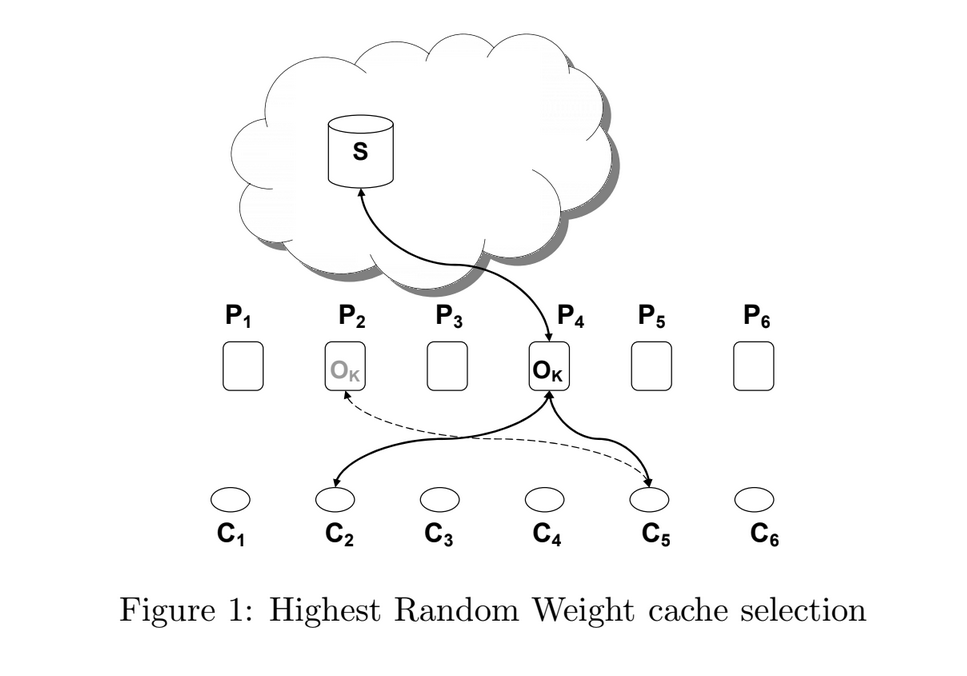
\includegraphics[height=2.3in]{HRW.PNG}
%\epsfig{figure=hrw.eps,height=2.5in,angle=-90}
\caption{Highest Random Weight cache selection\label{fig:hrw}}
\end{center}
\end{figure}

\subsection{Highest Random Weight Hashing}
Let there be a set of proxies $P_1, P_2,\ldots, P_n$ that retrieve and cache
objects from a remote server.  Let us say that clients $C_1, C_2$, and $C_3$
all want to retrieve the same object (a file) $O$.  If $C_1$ asked for $O$ from
proxy $P_{k1}$, $C_2$ asked for it from $P_{k2}$, and $C_3$ asked for it from
$P_{k3}$, there would be misses at $P_{k1}, P_{k2}$, and $P_{k3}$. On the other
hand, if $C_1, C_2$ and $C_3$ were to all ask for $O$ from the same proxy, say,
$P_k$, the first request for $O$ would cause $O$ to be retrieved from the
remote server, and cached at $P_k$. Later requests would therefore see a hit
at $P_k$ for $O$. A strategy that allows all clients to go to the same server
for a given object is called a \textit{consistent hashing} scheme.

You are to implement the Highest Random Weight scheme for consistent hashing.
Clients first concatenate the object name with the proxy name for each of the
$n$ proxies, and hashing these $n$ resulting strings to get $n$ hash values.
A client requests object $O$ from the proxy $P_k$ that yields the highest
hash value. Since all clients see the same proxies, the highest hash value
for $O$ will result at all clients from the same proxy name.

\subsection{Bloom Filters}
Bloom filters are probabilistic data structures used to answer set approximate membership queries.
A bloom filter $F$ consists of $m$ cells and $k$ hash functions $h_1, h_2, \ldots, h_k$.
Two operations are allowed:
\begin{itemize}
\item To \emph{insert} an item $x$ to $F$, we update $k$ cells at indexes $h_1(x), h_2(x), \ldots, h_k(x)$.
\item To \emph{query} if an item $y$ is present in the set of elements that have been inserted in $F$, we 
check cells at indexes $h_1(y), h_2(y), \ldots, h_k(y)$ for updates. If at least one cell is found to be updated, 
the element is \textit{probably} present in the set, otherwise, the element is definitely not.
\end{itemize}

Note that due to hash collisions, bloom filters may have \textit{false positives}, i.e.
a query may return `yes' even for elements that are not present in the set. However, no false negatives
are allowed, i.e. if a query returns `no', the element is definitely not in the set.

Each proxy server $P_i$ should maintain a bloom filter $F_i$ to check if the $P_i$ has seen a file request in the past. If the request has been fulfilled in the past, $P_i$ should return the file from its cache, or retrieve the file from the remote server otherwise. You may assume that a proxy never deletes cached objects.

% \section{Using TLS}
% The client and proxy $P_k$ will establish an TLS connection.  The client
% authenticates itself using a digital signature and message digest. The proxy
% verifies the client's identity, and checks to see if it has the requested
% object in its cache.  If it does, then the proxy will generate the hash value
% for each block of text, encrypt both the block and its hash using the client's
% RSA public key and then send it to the client through the TLS connection.

% If the proxy does not have the requested file in its cache then it establishes
% an TLS connection with the remote server to retrieve the file.  As with the
% connection between the proxy and the client, the proxy authenticates itself
% by using a digital signature and message digest. After verifying the proxy's
% identity, the server generates a hash value for each block of text, 
% encrypts both the block and its hash using the proxy's RSA public key, and
% sends it to the proxy through the TLS connection.  Once the file arrives at
% the proxy, it can be cached and forwarded on to the client as discussed
% above.

\section{Implementation details}
The starter code given to you is the same as one handed out in the labs. You are given a simple client and server that communicate in plaintext over a socket. libtls is included in the given repository. You are to use the libtls C API to make the client, the proxy servers and the remote server use TLS for all connections. Please read through the included README.md and the lab assignment for more hints on implementation details.

% To implement the project you will work in teams of two student using the C/C++ 
% programming language.  For all cryptographic tasks you should use the 
% OpenTLS security library including the SHA1 implementation and RSA 
% implementation included in the OpenTLS package. OpenTLS is a software library 
% that provides a full-featured cryptographic toolkit as well as an 
% implementation of TLS. The Unix version, which we will be using, provides 
% two libraries, one for TLS/TLS (ssl) and one for the cryptographic toolkit 
% (crypto) as well as command-line tool (openssl).  The OpenTLS Project's Web 
% page, http://www.openssl.org , contains HTML versions of much of the OpenTLS 
% documentation, as well as links to FAQs and other documents available on the 
% Web about using OpenTLS. You can also download your own copy of OpenTLS. 
% The RSA implementation is a part of OpenTLS package.  Since OpenTLS's 
% documentation of parts of the Crypto library are lacking, Ariel Glenn's 
% documentation of TLSeay (the precursor to OpenTLS) at 
% (http://www.columbia.edu/$\sim$ariel/ssleay/) may be of particular help.  


\subsection{Client side steps}
The client executes as follows.
\begin{enumerate}
\topsep=0pt\itemsep=0pt
\item
Determines the identity of the proxy to contact to retrieve a particular
file by computing a hash of the filename and the proxy name. 
\item
The client initiates a TLS handshake with the proxy.
(you may assume that the client already has a CA root certificate (\textit{root.pem}) required to authenticate the server)
\item
Sends the filename securely to the proxy
\item
Receives and displays the contents of the file requested.
\item
Closes the connection.
\end{enumerate}
\topsep=0pt\itemsep=0pt

The client application should be executed as follows:

       \qquad{\tt your\_application\_name -port proxyportnumber filename}

\subsection{Proxy side details}
The proxy executes as follows.
\begin{enumerate}
\topsep=0pt\itemsep=0pt
\item
Waits for the client to initiate a TLS handshake.
\item
Receives a request for filename from the client through the TLS connection.
\item 
Checks if the file has been requested in the past by querying the bloom filter for filename.
\item 
If the bloom filter returns `yes', the file may have been requested in the past, and it might be present in the cache. If the file is present in the cache, read in the file and send it to the client over TLS. Then add the filename to the bloom filter.
\item 
If the bloom filter returns `no' or if the file is not present in the cache, set up a TLS connection to the server , request for the filename and store it in the cache. Then read in the file and send it to the client over TLS. Finally, add the filename to the bloom filter.
\item
Closes the connection.
\end{enumerate}

The proxy application should be executed as follows:

        \qquad{\tt your\_application\_name -port portnumber
		-servername:serverportnumber}

\subsection{Server side details}
The server executes as follows.
\begin{enumerate}
\topsep=0pt\itemsep=0pt
\item
Wait for a proxy to initiate a TLS connection.
(You may assume that all proxies already have the CA's root certificate (\textit{root.pem}) required to authenticate the server).
\item
Receives a request for filename from the proxy through the TLS connection.
\item
Sends the file securely to the proxy over the TLS connection.
\end{enumerate}

The proxy application should be executed as follows:

        \qquad{\tt your\_application\_name -port portnumber}


\section{Requirements}
\begin{enumerate}
\topsep=0pt\itemsep=0pt
\item All applications should:
\begin{enumerate}
\topsep=0pt\itemsep=0pt
        \item display console messages after each step
        \item check errors during the communication of the two parties and 
          display appropriate message indications for the specific error 
          identified prior, during and after the connection
\end{enumerate}
\item Since you will most likely be implementing the clients, proxies and server
all on the same machine please organize the information for each client, proxy
and the server in a separate directory on the file system.
\item You should use C to implement your application, and your code 
should be clearly written and well documented. Using C++ is allowed, but please remember that calling C code from C++ and vice versa may not be straightforward due to linking issues. You might want to look up the "extern C" directive. Please write a README file with your code. You should turn in your code on iLearn.
\item Although you are allowed work in pairs to complete this 
assignment the assignment should be the {\it original work\/} of the team. 
You might discuss the concepts and the libtls library with other students but 
sharing the code between teams will result in you failing the assignment. 
We will use automated tools to check for cooperation. 
\end{enumerate}

\section{References}
\begin{enumerate}
\item \href{https://github.com/bob-beck/libtls/blob/master/TUTORIAL.md}{Bob Beck's libTLS tutorial.}
\item \href{http://www.openbsd.org/papers/linuxconfau2017-libtls/}{LinuxConf AU 2017 slides.}
\item \href{https://jamielinux.com/docs/openssl-certificate-authority/introduction.html}{On Certificate Authorities.}
\item \href{https://man.openbsd.org/tls_init.3}{Official libtls documentation}
\end{enumerate}

\end{document}
